\documentclass[12pt]{article}

\usepackage{hyperref}
\usepackage{titlesec}
\usepackage{amsthm,amssymb}
\usepackage{amsmath}
\usepackage{graphicx}
\usepackage{minted}

\graphicspath{ {images/} }

\title{CS3210 Assignment 1 Part 2 Report}
\date{\today}
\author{Mok Wei Xiong, Edmund (A0093960X)}

\begin{document}
% title
\maketitle

\section{Program Design}

\subsection{General Description}
\subsubsection{OpenMP version}
In my design, a train is represented by a thread. If there are $n$ trains in total for all green, yellow and blue lines, then there will be $n$ threads representing the trains. Additionally, in the simulation, I will also have $1$ thread (the master thread) that does not represent any train, but is in charge of printing the state of the trains at every tick. Thus, during the simulation, if there are a total of $n$ trains in the system, there will be $n+1$ threads.

\bigbreak \noindent Every thread is in charge of only $1$ train, and controls that train throughout the entire simulation. Each thread will loop for $N$ iterations, where each iteration represents a tick. In each iteration, each thread will attempt to load people into the train, move along a track, or just do nothing if it is waiting for another train in front of it. Named critical sections are used as mutexes to prevent race conditions by trains waiting for the same station, or trains waiting for the same track. FIFO Queues are similarly used at each station and track to prevent starvation, by guaranteeing that any train that is queued will be eventually served.

\subsubsection{MPI version}
In the MPI version, each (unidirectional) link and station is represented by a process. Unidirectional links shared between multiple lines are considered as one link and is represented by one process. If there are $p$ unidirectional links, $q$ stations, then there will be a total of $p+q+1$ processes, including 1 master process for doing coordination. As before, each process will do 1 simulation tick on its own, then wait at a barrier for all processes to finish that tick, then go on to simulate another tick until the desired number of ticks have ran. Once again, FIFO queues are used at stations and links to prevent starvation. No critical sections are required since each process is in charge of its own queue.

\subsection{Assumptions}
\begin{itemize}
	\item We are given that only one train can load at a station (in any direction) at any time. Direction is not taken into account because it is impossible to make it consistent since one line's "forward" direction is not the same as another line's "forward" direction. There can be multiple trains waiting at a station. Once the first train is done loading, it may possibly still have to wait for another train on the track in front of the station before it is allowed to leave. I assume that the train behind can be allowed to start loading, meaning it can open the door to load passengers, even though the first train may still be waiting for the track.
	\item The definition of \textbf{average waiting time} given in the assignment handout is not very clear on whether the average waiting time is (A) the average of all individual average waiting times of each station on a line, or (B) the average of \textit{all} waiting times experienced by every station on the line. I have chosen to take approach (B) for my implementation.
\end{itemize}

\section{Implementation Details}

\subsection{Stations on a line}

The input format given specifies three lines $G, Y, B$, with each line containing a list of stations separated by commas to indicate the stations that are served by each of the lines. The sample format nicely specifies each list of station in "order", where the terminal stations are at the start and end of the list, and the stations in between connect the two terminals. For example, the input format specifies, for the yellow line, \verb!tuas, clementi, tampines, changi!, which is a right "order" for the line, whereas an input format that does not specify a right order is something like \verb!clementi, tampines, tuas, changi!.

\bigbreak \noindent In my implementation, I assume that all inputs given have the right "order" to simplify the IO part of the program since it is not really the main focus.

\subsection{Integer loading times}

The input popularities for each station is specified as a floating point number, which means that the loading times should also be a floating point number. However, the simulation works in discrete time ticks, so it would not be possible to perform actions like stopping the train from loading between two integer time ticks, once the loading time is up. Thus, I took the ceiling for each loading time computed using \verb!ceil! so that the train will always wait at least the correct amount of time to load.

\subsection{Queueing trains}

At every station and every track connecting two stations (in a single direction), there will be a queue. Trains must queue up to load passengers, or to start moving on a track using the respective queues before they are allowed to take action. They can only take action when they are at the front of the queue.

\bigbreak \noindent This queue prevents starvation since the moment any train arrives at a station or a track, it is immediately enqueued into the appropriate queue and waits for its turn in the queue. Since the train at the front of the queue will eventually complete, since there is a limit to the time the train at the front of the queue can load passengers or move across a track, it will eventually be removed from the front of the queue. This means every train in the queue will eventually reach the front of the queue where it is then allowed to execute its appropriate action, and thus there will not be starvation!

\section{Implementation Specifics (OpenMP version)}

\subsection{Train threads}

As mentioned, for every train in the simulation, there will be a thread that is spawned and in charge of that train throughout the entire simulation. Before the simulation, a vector of \verb!Train! objects are created, and the master thread will feed appropriate information into each \verb!Train! so that later during the simulation, each thread will know the current state of its \verb!Train! using only its allocated \verb!Train!. Examples of what each \verb!Train! contains include what line it is in, the train number, the stations in this line, the direction it is moving in, and whether it is currently loading or moving. The \verb!thread_id! of each thread is used to identify the \verb!Train! that the thread is assigned to.

\bigbreak \noindent The threads are created using \verb!#pragma omp parallel num_threads(n + 1)!, where n is the total number of trains in the system. There is an additional $1$ thread that will not be in charge of any train and simply prints the state of every train at each tick.

\subsection{Synchronization}

\subsubsection{Printing state}

\begin{minted}{C++}
  #pragma omp parallel num_threads(train_counts.num_total + 1)
  {
    // master will occupy thread_id = 0, so offset all workers by 1
    int thread_id = omp_get_thread_num();
    int train_id = thread_id-1;

    // Run for max_tick number of times
    for (int tick=0; tick<max_tick; tick++) {

      // First let master print out the current state of the system
      #pragma omp master
      {
        print_system_state(trains, tick);
      }

      // Let master finish printing before all trains make their moves
      #pragma omp barrier

      // All trains make their move for this tick
      // (except master thread who does not own a train)
      if (thread_id != MASTER_THREAD) {
        Train& train = trains[train_id];
        assert(train.gnum == train_id);
        simulate_train(train, tick);
      }

      // Let all trains wait for master to print their state
      #pragma omp barrier
    }
  }
\end{minted}

\bigbreak \noindent The above code snippet shows the synchronization structures used to ensure that there is no race condition when the master thread attempts to print the state of the system in the current tick.

\bigbreak \noindent In each tick, the master thread will always get to print the system state before every other train makes its move for the current tick. This is ensured by the usage of the \verb!#pragma omp barrier! after the code used to get the master to print the system state within \verb!#pragma omp master!. Only when the master has completed printing the state, will all the threads pass through the first barrier. After that, every train will make its move for the current tick using \verb!simulate_train!. Another \verb!#pragma omp barrier! is placed at the end of the current tick to make sure all trains have finished making their move for the current tick before proceeding on to the next tick, to prevent race conditions.

\subsubsection{Synchronizing queues}

Since we are using the front of the queue to determine whether the train is allowed to take action, there is a possibility of a race condition, affecting the outcome depending on whether the train at the front of the queue executes before the train just behind the front of the queue, or after. In order to avoid this race condition, I use a \verb!#pragma omp critical(name)!, to act as a mutex so that only one thread interested in \verb!name! can manipulate the queue at any time. In the case of station mutexes, \verb!name! is the station number. In the case of track mutexes, \verb!name! is a concatenation of the \verb!source! station and the \verb!destination! station.

\section{Implementation Specifics (MPI version)}
\subsection{Trains as messages}
In the MPI version, since we had to implement tracks and stations as processes, then in order to move the trains around the tracks and stations, we need to use the message passing in MPI. Each track and station manages a queue of trains, and keeps track of a countdown timer for the train at the front of the queue (whether it is time left to load or remaining time on track to reach next station). 

\bigbreak \noindent At every tick, each process (both station and tracks) will first decrease remaining time for the train at the front of their queue (if there is one). If the train has run out of time, it needs to be passed on to the next station or track immediately after this. 

\bigbreak \noindent Every station will send a message to all its neighbours indicating whether there is a train to pass onto the neighbour. This message can either be a real message representing the serialization of a real train (like train line, train number), or a dummy message. At the same time, every track will do a receive operation, and wait to receive a message from the neighboring station. This is to prevent deadlock in case the \verb!MPI_Send! does not actually return for some reason, such as if there is no write buffer and the send actually needs to be received by the neighboring process.

\bigbreak \noindent After all sends are completed by the stations, they will do a "receive" from each of its neighbors (the tracks), and the tracks will all do a send after completing their receive. If a train should really move on to the next station or track, a real message will be received, otherwise a dummy message will be received and the receiver process will just ignore it.

\bigbreak \noindent Also, at the start of every tick, all stations and tracks will send information of all trains in their queues to the master process. The master process will then use information about the trains to print the status of the trains at each tick. At the end, every station will send timing informations of each station (like total wait time, min and max waiting time) to the master process, which will aggregate the results and print the final output.

\subsection{Serializing objects as messages}

As far as I know, MPI only allows messages containing a fixed set of data types, such as \verb!MPI_INT!. Since I had some data stored in \verb!struct! types, such as the \verb!Train!, I had to explicitly create a new \verb!int! array and put in information from the \verb!Train! to be sent in \verb!MPI_Send!, and reconstruct the \verb!Train! after receiving the \verb!int! array from \verb!MPI_Recv!.

\subsection{Enforcing number of processes}
In MPI, when we do a \verb!mpirun!, we can actually specify the number of processes before the the program is even run. Since the assignment requirement is that each link must be represented by a process (and also stations), this needs to be enforced somehow but can only be checked when the input has been read. I do this check immediately after the input is read, and terminate the program if the number of processes used during \verb!mpirun! is not the correct number (depends on the input).

Due to the way I tried to implement the checks, I basically read the input file twice, the first time to check whether the number of processes used is \textbf{correct}, and the second time to setup for the actual simulation. Furthermore, I restrict the input file to be only \verb!in.txt!, instead of allowing input redirection like for the OpenMP version.

\section{Simulation Ticks vs Execution Time}

This implementation of the simulation used discrete time units (ticks) instead of running based on execution time.

\bigbreak \noindent There are several advantages of this approach:
\begin{itemize}
	\item Waiting times do not depend on CPU power when using ticks. For every tick, waiting times do not depend on how fast the CPU takes to execute that tick. This means that we can compare waiting times across different CPUs, and even different number of threads on the same CPU (especially very large number of threads for very large number of trains), because the context switching will not impact the waiting times. As can be seen from the difference in execution times between the OpenMP and MPI versions, simulation ticks are definitely a fairer way to compare between different "routing of lines" in practice, since execution time will depend on the resources (like number of trains affecting number of threads in OpenMP version, and number of links and stations affecting number of processes in MPI version).
	\item Ease of implementation. Implementation is easier when every thread only needs to deal with a single tick, and determine what it should do during that tick. If ticks were not used, we may need things like sleep timers (for example, to sleep until the load time at a station has expired, or to sleep until the train has completed using a track), or more synchronization primitives like condition variables (to know when the train ahead has finished loading, or finished using a track, and the next train can start doing something). With ticks, we can just check if these conditions are met in the current tick.
	\item Simulation time units are also not affected by \verb!IO!, which occurs quite frequently in this simulation (every tick the master thread does some \verb!IO! to print the state of the syem).
\end{itemize}

\bigbreak \noindent However, there are also downsides:
\begin{itemize}
	\item Since the popularities of each station can be a floating point number, according to the loading time formula, the loading time for a train can also be a floating point number. However, since the simulation uses single integer ticks, the simulation will force the train to continue loading until the next nearest integer (ceiling), which means that the simulation will lose its accuracy here when computing the average, minimum and maximum waiting times.
\end{itemize}


\section{Execution Times (OpenMP version)}

Each execution time result is obtained by running the programme $5$ times, and taking the minimum execution time across all runs. All runs were executed on Dell Precision 7820 with Intel Xeon. Each run used the same system as provided in the assignment handout, but with $N$, the number of time-ticks for the simulation set to $1000$. The program was compiled using \verb!g++ -std=c++11 main.cpp -fopenmp -O3 -o main!, and each test case was placed in a file \verb!example.in! in the same directory. Each run was executed by using \verb!time ./main < example.in!, and the resulting \verb!real! time output was considered as the execution time.

\begin{table}[]
\begin{tabular}{|l|l|l|}
\hline
Number of trains & Composition (G,Y, B) & Execution Time (seconds) \\ \hline
1                & 1, 0, 0              & 0.015                    \\ \hline
2                & 1, 1, 0              & 0.016                    \\ \hline
3                & 1, 1, 1              & 0.017                    \\ \hline
6                & 2, 2, 2              & 0.023                    \\ \hline
10               & 3, 3, 4              & 0.042                    \\ \hline
15               & 5, 5, 5              & 0.053                    \\ \hline
18               & 6, 6, 6              & 0.054                    \\ \hline
19               & 7, 6, 6              & 0.082                    \\ \hline
20               & 7, 7, 6              & 0.173                    \\ \hline
25               & 8, 8, 9              & 0.22                     \\ \hline
30               & 10, 10, 10           & 0.259                    \\ \hline
35               & 12, 12, 11           & 0.313                    \\ \hline
40               & 14, 14, 12           & 0.335                    \\ \hline
50               & 16, 16, 18           & 0.45                     \\ \hline
64               & 20, 20, 24           & 0.593                    \\ \hline
\end{tabular}
\caption{Result of OpenMP execution time across number of trains}
\end{table}

\begin{figure}
	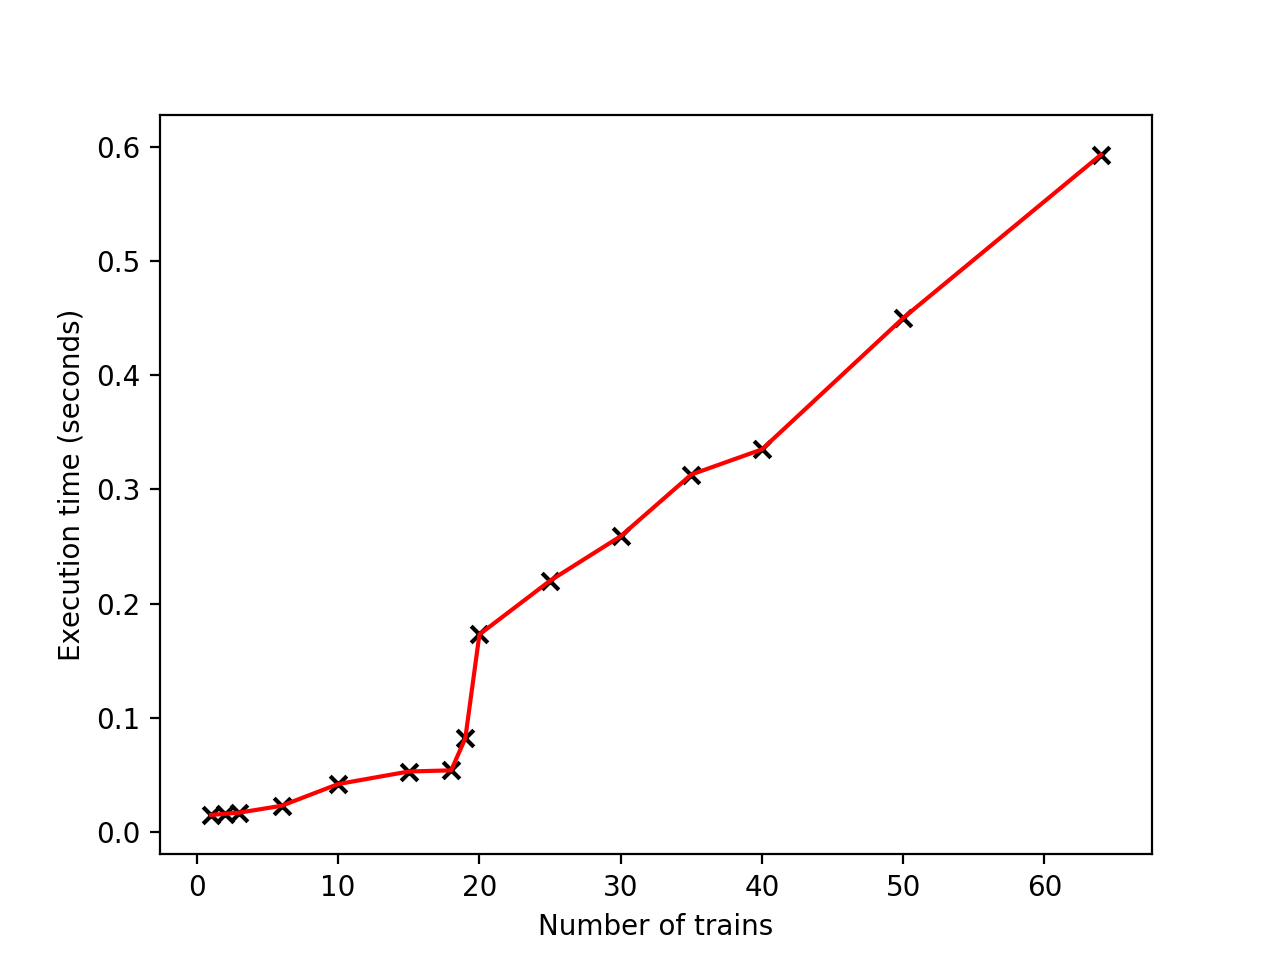
\includegraphics{execution_times}
	\caption{Plot of execution time across number of trains}
\end{figure}

\section{Result Analysis for OpenMP version}

\subsection{General trend}

In general, from the plot and the table, we can observe that the execution times increase with increasing number of trains (threads). 

\bigbreak \noindent There are a couple of possible reasons for this:
\begin{itemize}
	\item More trains means more context switching between different threads, which leads to overhead resulting in higher execution time.
	\item More trains means that the master thread needs to loop through more trains in each tick to print out more train states during each tick. This means that there is more \verb!IO! with increasing number of threads, which can be quite slow and thus lead to greater execution times.
	\item More trains means more competition for critical sections. If a thread fails to enter a critical section, it has to wait until it gains access before it can proceed with the rest of the code. Since more competition for critical sections results in a higher chance of failure in gaining access to critical sections, more threads are delayed in completing their work for the current tick, thus increasing execution times per tick, and hence over the entire simulation.
\end{itemize}

\subsection{Mysterious Spike}

Besides the general increasing trend, we can notice an obvious mysterious spike in execution time at around $20$ trains, or $20$ threads. I suspected that it had something to do with the number of cores on the Intel Xeon processor, and the maximum number of threads the Xeon processor could handle optimally. Even if the Intel Xeon had multiple cores, the general advice is to have a maximum of $2$ threads per core for optimal performance before the increasing number of threads begins to hurt performance.

\bigbreak \noindent I referred to Part 2 of Tutorial 1's handout, where we were given a diagram of the workbench cluster. In the diagram, specifications of the Intel Xeon used were given - 10 cores (20 threads)! Just as I had suspected, beyond 20 threads, the Xeon processor cannot perform as well as the number of threads per core started becoming suboptimal. 

\bigbreak \noindent The last observation is that the rate of increase after the spike is greater than before the spike. I think the possible reasons for this are similar to before: the overhead in context switching between threads, the greater competition for critical sections between threads.

\section{Execution Times (MPI version)}

Each execution time result was obtained by running the programme $5$ times, and taking the minimum execution time across all runs. All runs were executed on Dell Precision 7820 with Intel Xeon. Two different "map" layouts were used, one smaller version with only four stations with links connecting all of them like a connected graph that required 17 processes, and the default map given in the handout which required 25 processes in total. Different maps used was to vary the number of links, which then varies the number of processes as required in the assignment. All maps used a fixed 10 trains for each line, so a total of 30 trains, and all ran for 1000 ticks.

\bigbreak \noindent For each map type, number of cores were varied, for 1, 2, 4, 8, ..., until 28 cores. The number of cores was set by using the \verb!-machinefile! flag set to an appropriate machine file and the \verb!-rankfile! set to an appropriate rankfile. The files used are attached with the rest of the code. For example, for 2 cores, every rank \verb!i! was mapped like \verb!rank i=soctf-pdc-006 slot=0:0-1! to restrict it to cores [0, 1].

\begin{table}[]
\begin{tabular}{|l|l|l|}
\hline
Number of cores & Small Map (17 processes) & Default Map (25 processes) \\ \hline
1                & 0.686              & 0.712                    \\ \hline
2                & 0.457            & 0.722                    \\ \hline
4                & 0.353              & 0.572                    \\ \hline
8                & 0.284              & 0.423                    \\ \hline
10               & 0.266              & 0.494                    \\ \hline
12               & \textbf{2.023}              & \textbf{2.351}                    \\ \hline
16               & 2.034              & 2.355                    \\ \hline
20               & 2.007              & 2.343                    \\ \hline
24               & 1.943              & \textbf{2.778}                    \\ \hline
28               & 1.873              & 2.722                    \\ \hline

\end{tabular}
\caption{Result of MPI execution time (in seconds) across number of processes and cores}
\end{table}

\section{Result Analysis for MPI version}

In general, from Table 2, we can observe that the execution times decrease with increasing number of cores, up to a certain point Increasing number of cores means that more processes can run in parallel, especially since the MPI version relies heavily on processes running each tick until the desired number of ticks.

\bigbreak \noindent Another observation is that increasing the number of processes, while the number of cores remains constant, causes the execution time to increase. This is also obvious, and the reasoning is similar to above, since there are more processes, there is more competition for the limited number of cores and so the processes will take longer to complete and so execution time will increase.

\bigbreak \noindent There was also a weird outlier at 10 cores and 25 processes, where increasing the number of cores from 8 to 10 actually increased the execution time. I'm not too sure what caused this, as repeated time measurements yielded around the same results (timing increased compared to 8 cores). One possible explanation could just have been randomness in measuring the timings.

\bigbreak \noindent As mentioned earlier, after a certain point, increasing the number of cores increases the execution time on both maps (number of processes). For example at the transitions between 10 $\rightarrow$ 12 cores and 20 $\rightarrow$ 24 cores, the execution time can be seen to increase. The reason is simple, because when for example the number of cores increase from 10 $\rightarrow$ 12, I had to run the test on two Xeon processors instead of only a single processor, since a single Xeon processor had only 10 cores. As such, the communication time in sending and receiving messages increases by a lot, and multiplied by the number of messages sent and received in the entire run of 1000 ticks causes the execution time to increase a lot. The same thing happens for 20 $\rightarrow$ 24 cores, where I had to increase number of Xeon processors from 2 to 3, which increases communication time once again.

\bigbreak \noindent Thus, increasing number of cores does not always lead to better execution times if they communication overhead increases due to the cores being on separate machines.

\section{Execution Times (OpenMP vs MPI)}

Each execution time result was obtained by running the programme $5$ times, and taking the minimum execution time across all runs. As with the MPI version, all runs were executed on Dell Precision 7820 with Intel Xeon using two map types.

\bigbreak \noindent For each map type, the number of trains was varied when testing both OpenMP and MPI versions. In total, the number of processes and threads were varied and measurements were taken.

\begin{table}[]
\begin{tabular}{|l|l|l|}
\hline
Map Type & OpenMP & MPI   \\ \hline
Small    & 0.005  & 0.176 \\ \hline
Default  & 0.007  & 0.23  \\ \hline
\end{tabular}
\caption{Result of OpenMP vs MPI execution time (in seconds) at 0 timeticks}
\end{table}

\bigbreak \noindent First of all, I made some initial measurements setting the number of timeticks executed at 0. This allows me to measure how much time is spent sending messages and setting up the data in the processes by message passing in the MPI version compared to the OpenMP version, which uses shared memory. As can be seen in Table 3, around 0.1 - 0.2 ms alone was already spent on just trying to send messages to setup for the simulation instead of performing the simulation itself! In my implementation, only the master reads from the input and has access to all the data at the start, so quite some messages need to be sent from the master to all the other processes.

\begin{table}[]
\begin{tabular}{|l|l|l|l|}
\hline
Map Used & Number of trains & OpenMP  & MPI                    \\ \hline
\textbf{Small}                & 10                & 0.028                & 0.217                    \\ \hline
                & 20                     & 0.152            & 0.248                    \\ \hline
                & 40                    & 0.349          & 0.262                    \\ \hline
                & 64                     & 0.557          & 0.319                     \\ \hline
\textbf{Default}                    & 10              & 0.03         & 0.357                     \\ \hline
                & 20            & 0.157            & 0.432                    \\ \hline
                & 40              & 0.315          & 0.465                    \\ \hline
                & 64              & 0.586          & 0.542                    \\ \hline
\end{tabular}
\caption{Result of OpenMP vs MPI execution time (in seconds) at 1000 timeticks}
\end{table}

\bigbreak \noindent From Table 4, we can see that the OpenMP version is faster for smaller number of trains while the MPI version starts to become faster when there is greater number of trains. This is not surprising since in the OpenMP version the number of trains controls the number of threads executing, whereas the number of trains does not affect anything other than the number of objects in memory in the MPI version.

\bigbreak \noindent Another unsurprising observation that can be made from Table 4 is that the larger maps increase execution time for MPI version but tdoes not really affect the OpenMP version much. Of course, since the map type affects the number of stations and links which affects the number of processes in MPI but does not affect anything much in the OpenMP version, this observation is expected.

\subsection{Conclusion}

In my opinion, the OpenMP version is probably a \textit{better} way to simualte the train network in most cases. The OpenMP version relies on threads to move the trains directly whereas the MPI version relies on processes for the links and stations to handle the movement of trains with each other. In most train networks, the number of trains is usually much smaller than the number of stations and links, so the \textit{resources} required in the simulation would be smaller and the overhead in context switching would likely be smaller, leading to faster execution times. Even if the MPI version can be run across a huge number of cores, the increase in communication time across multiple machines would not be "worth" at all. Even though the OpenMP version required synchronization to prevent race conditions, it was much easier to implement than trying to send and receive messages between different processes.


\section{Bonus}

As mentioned before, I believe that my implementation will never encounter starvation since every train that wants to wait for a resource will be doing so in a queue, and train will always reach the front of the queue eventually. As a result, the train will eventually get to execute its action and will never starve. The train at the front of the queue will always leave the queue eventually because the time it can be at the front of the queue is finite and bounded, so trains at the back of the queue can eventually move to the front.

\end{document}
